\chapter{Measuring Items' Behavioural Change}
\label{Chap:Measuring}

 
 \section{Introduction}
 
 This chapter addresses the research questions raised in chapter one regarding the use of clustering and cluster validity indices as a method to measure items behaviour through multiple time points. The questions and hypothesis will be tested using the methods mentioned in Chapter three Section \ref{MeasuringChangesOverTime} and related to items' behaviour measurement in temporal data.
 
 The Hypothesis \ref{hypo:diffCluster} in chapter one indicates that the result of quantifying the behavioural change will not be affected by using various clustering algorithms as long as all time points are clustered using the same algorithm. To test this hypothesis, we use multiple clustering algorithms like k--means, c--means, PAM and hierarchical clustering in this chapter to cluster the temporal data. Each clustering algorithm is used to cluster all time points of the temporal data set separately from each other and without the effect of the time attribute.
 
 Hypothesis \ref{hypo:diffCVI} indicates that different external cluster validity indices will produce similar results in measuring items' behavioural change between the various time points. To check the validity of this hypothesis, we used different external cluster validity indices to measure changes between any two time points. However, not all external cluster validity indices might be suitable to be utilised for this task as we, later in this chapter, will explain the essential characteristics of the measure which can be used. Moreover, we have used Area Under the Curve AUC of ROC analysis to measure changes over time for comparison purposes with external cluster validity indices.
 
 This chapter also partially addresses the reference of behaviour for items in temporal data (Hypothesis \ref{hypo:overallBehavoiur}). Reference of behaviour can be defined as a typical collective behaviour of elements of a temporal data set. Reference of behaviour can be used to compare other time point behaviours of items. In this chapter, we will use and test two different Reference of behaviours for items. However, after we introduce the proposed temporal classification method in the next chapter, we will use it to classify items in the data sets and use these classes as a reference of behaviour for all time points.
 
 Three data sets are used in our tests one synthetic data set to check the feasibility of using the proposed method as a measure of quantifying change over time and two different public goods games PGG data sets (as mentioned in chapter three, section  \ref{PublicGoodsGamesData}). Moreover, this chapter participates in the argument of the players' strategy change during the PGG rounds \cite{Chaudhuri2010, Fischbacher2009} by presenting a quantifiable method to measure the change in strategy by players.
 
 
 Finally, the results are compared with the MONIC model as it developed by Spiliopoulou et al. \cite{Spiliopoulou2006} to measure the cluster changes in the data streams (Further details on the MONIC method are provided in chapter two). The appropriate statistical analysis is presented to provide evidence supporting or rejecting the hypotheses of the first chapter.
 
 \section{Background}
 In economics, there is an interest in how players of public goods game change their strategy during multiple rounds of the game and jump from one strategy to another \cite{Fischbacher2010}, such as changing from conditional cooperator to free rider behaviour. This change can be seen as a drift from the original label assigned to the players.
 
 There are many methods for classification in machine learning, with the existence of concept drift \cite{Elwell2011,Garnett2008,Xiaofeng2014} and methods to detect it \cite{Baena-Garcia2006,Harel2014}. Moreover, measuring changes in clusters for different time points have been thoroughly studied in data analysis, especially for data streams \cite{Ntoutsi2011,Spiliopoulou2013,Yang2011}. However, these methods aim to find overall patterns of change in clusters' location, size, merging, emerging and/or dissipating rather than presenting a measure of how much change has occurred in each cluster (that is, in which ratio items change their membership from one cluster into another).
 
 External cluster validity is primarily used to check the performance of clustering algorithms by measuring the difference between ground truth labels given to the items by experts and the group in which they have been placed by a clustering algorithm \cite{Halkidi2002a}. This study uses external cluster validity measures such as variation of information \cite{Meila2003} VI and area under the curve of the receiver operating characteristic AUC \cite{Bradley1997} as scaler measures, to show the magnitude of items that jumped from one cluster to another between two consequent time points. To accomplish this measurement the items should be clustered separately in every time point. As the clustering is performed at a single time point, which eliminates the time dimension for the collected data on items, any traditional (non-temporal) clustering algorithm should theoretically be sufficient. After clustering, an external clustering validity measure can quantify the amount of changes between clusters at any two time points.
 
 
 \section{Approach}
 As has been explained in the previous chapter, to be able to measure the difference in behaviour of a population of items from their collected characteristics in a temporal data, the items should be clustered in each time point. Then their change in behaviour can be measured using cluster validity indices CVI or Aria Under the Curve AUC of ROC analysis. However, to implement the available methodology on a specific data, certain decisions have to be made to ensure that appropriate treatments are applied to the underlying data. In the following sub-sections, the rationale and reasons for selecting data set attributes, choosing the number of clusters, clustering algorithms and various cluster validity indices is explained.
 
 
 \subsection{Preparing Data Sets for Clustering}
 Before starting with clustering, the temporal data sets have to be separated by their time points. In this chapter, three data sets are used for the tests. The first data set is the synthetic data set as mentioned in section \ref{CreatingaSyntheticData}. The second and third data sets are public goods game data sets with different players and various length of time points.
 
 The synthetic data set is straight forward as it has 20 time points. So, the data will be split into 20 separate data sets with each subset representing one time point. The subsets are labelled so that the order of consequent subsets are preserved. The data has two temporal attributes in each sub-data set representing x and y coordinates.
 
 The first public goods game data set has 10 time points as presented by the ''period'' attribute so that it will be split into 10 subsets of data sets with each containing 140 items as the number of players in this data set. The second data set contains records of 27 rounds for 128 players so that this data set will be split into 27 subsets with each containing information of 128 players at a particular time point (round of the game).
 
 Both public goods game data sets have multiple static attributes and do not contain any temporal information. These static attributes are Idsubj, b0 to b20, u and Predictedcontribution. The temporal attributes are contribution, belief and otherscontrib. However, the otherscontrib is not directly related to the players' behaviour. Thus it is also not used in the clusterings. The only two attributes used are players contribution and belief of P-Experiment as these two attributes reflect the players learning the process for the game and the change in their ideas and strategies as the game progresses through rounds.
 
 \subsection{Choosing Clustering Algorithms}
 \label{sec:ChoosingClusteringAlgorithms}
 As each of the produced subsets of data represents one time point of the temporal data set, each subset alone, therefore, does not carry any information about the time dimension. This means it is possible to use non-temporal clustering algorithms to cluster items in each subset of the temporal data sets.
 
 
 Clustering algorithms can be categorised according to their method of finding similarities between items in the data. These categories are partitional, hierarchical, density-based, grid-based and fuzzy clustering \cite{Halkidi2001}. However, the main clustering categories which we used are partition based clustering,  hierarchical clustering and fuzzy algorithms. For the tests in this chapter, we used k--means and PAM as methods of partitioning clustering, hierarchical clustering with Euclidean distance and c--means as fuzzy clustering. As we aim to find similarities between items according to their distance from each other, we, therefore, did not use density-based and grid-based clustering methods.  Please refer to chapter two for further details on these clustering algorithms.
 
To find similarities between items, clustering methods can use linear distance measures such as Euclidean distance or use non-linear kernels to cluster complicated patterns in the data items. In the tests, we only used linear distance-based clustering methods because the aim was to find the similarity in behaviour based on the overall proximity of the attribute values of items. For the same reason, we did not use density-based clusterings such as DBSCAN and grid-based clustering such as STING since these methods do not depend on the mutual proximity of cluster items to a centroid. This represents a behaviour category.
 
 \subsection{Choosing Number of Clusters}
 \label{sec:Choosing-Number-of-Clusters}
 Most of the clustering algorithms require the number of clusters as an apriori condition to cluster the underlying data. This might be a challenging task especially for the data sets as there are no known patterns to start with \cite{Jain2010a}. Economists have classified players of public goods game data sets used in this chapter into four classes \cite{Fischbacher2001}. However, as explained in chapter three, these classes are dependent on the static attributes of the data rather than temporal attributes.
 
 Numerous methods exist to estimate the appropriate number of clusters in the data \cite{Milligan1985, Yu2014}. We used the elbow method \cite{Ketchen} to determine the number of clusters in the temporal attributes of the PGG data sets. This method involves clustering the data set repeatedly with an incremental number of clusters and then calculating the sum of square error or variance of items within clusters. By plotting the produced values, an appropriate number of clusters for the underlying data can be found.
 
 We used the ten round game data set to find the number of clusters in the temporal attributes of the public goods game data. The data is split into ten subsets with each subset representing one time point. Each time point is clustered repeatedly using k--means clustering, starting with 2 clusters up to 15 clusters. The sum of square errors within each cluster is calculated and plotted. The results in Figure \ref{fig:elbowNumberOfClusters} indicates that there is no absolute number for clustering. However, four clusters might be an accepted number of clusters for the data. 
 
 \begin{figure}[!h]
     \hfill{\begin{minipage}{\dimexpr \textwidth-2\fboxsep-2\fboxrule}% maximum allowed
             \centering
             \subfigure{
                 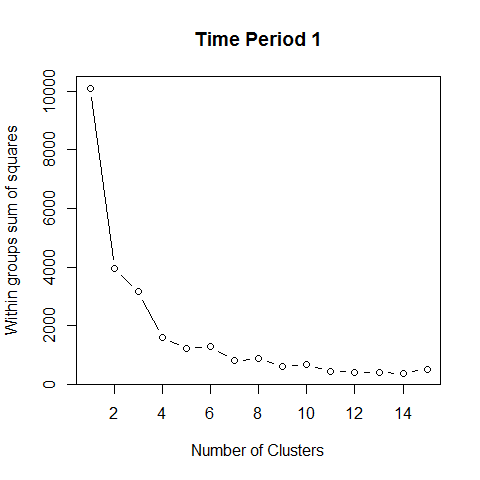
\includegraphics[width=0.32\textwidth]{images/chapter4/elbowNumberOfClusters1.png}
                 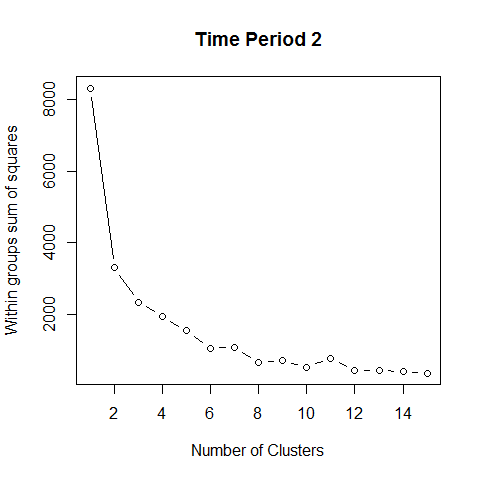
\includegraphics[width=0.32\textwidth]{images/chapter4/elbowNumberOfClusters2.png}
                 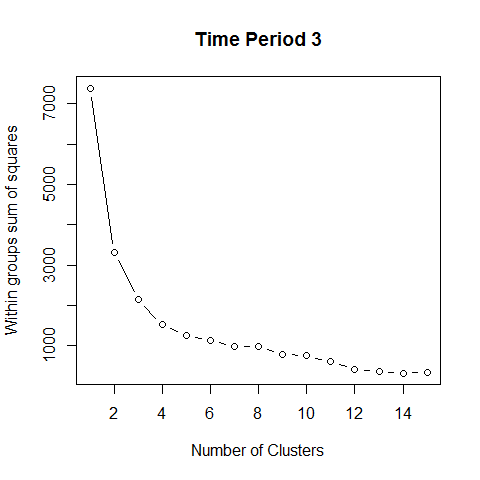
\includegraphics[width=0.32\textwidth]{images/chapter4/elbowNumberOfClusters3.png}
             }\\
             \subfigure{
                 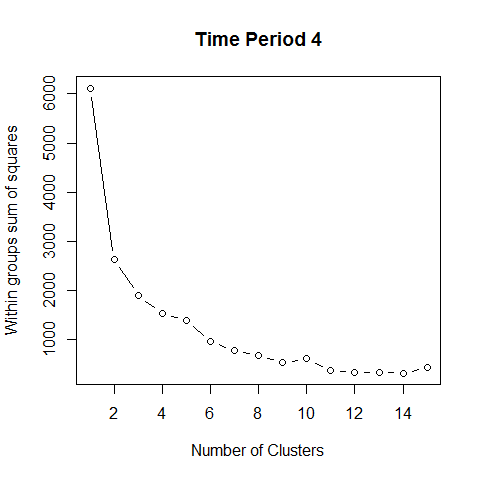
\includegraphics[width=0.32\textwidth]{images/chapter4/elbowNumberOfClusters4.png}
                 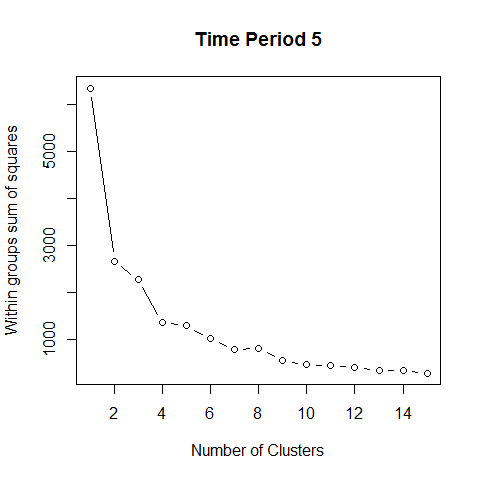
\includegraphics[width=0.32\textwidth]{images/chapter4/elbowNumberOfClusters5.png}
                 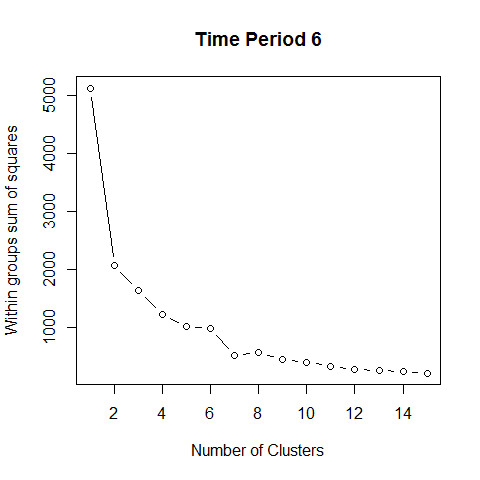
\includegraphics[width=0.32\textwidth]{images/chapter4/elbowNumberOfClusters6.png}    
             }\\
             
             \subfigure{
                 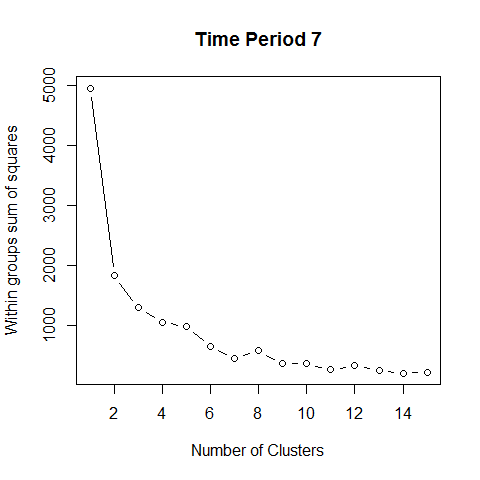
\includegraphics[width=0.32\textwidth]{images/chapter4/elbowNumberOfClusters7.png}
                 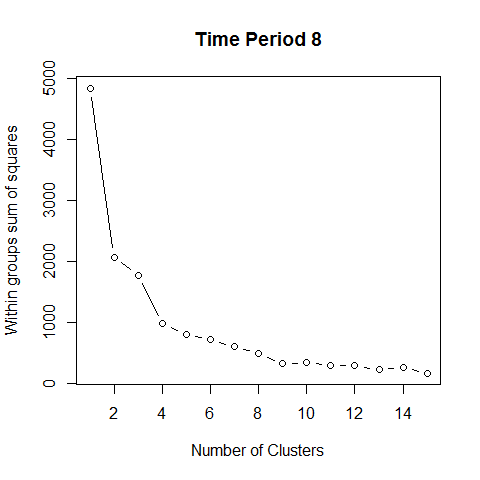
\includegraphics[width=0.32\textwidth]{images/chapter4/elbowNumberOfClusters8.png}
                 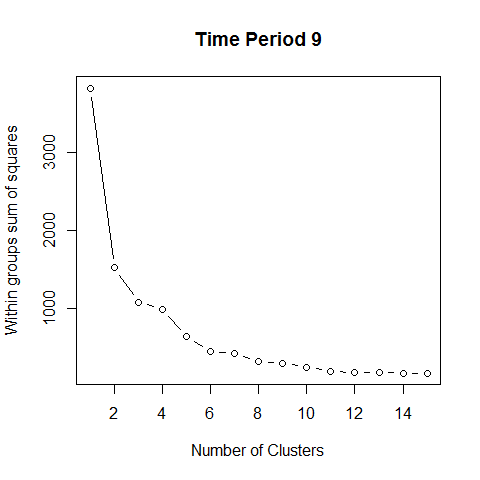
\includegraphics[width=0.32\textwidth]{images/chapter4/elbowNumberOfClusters9.png}    
             }\\
         \end{minipage}}
         \caption{Using elbow method and calculating the sum of squared errors within groups to find appropriate number of clusters for the public goods game data in each time point.}
         \label{fig:elbowNumberOfClusters}
     \end{figure}
     
     We implemented an extra test to evaluate the group memberships of players which are predicted by the clustering algorithm for cluster numbers from 2 to 15. Each of the previously clustering results was compared with economists' classifications using Rand external cluster validity. Please refer to chapter two for more information about Rand index for external cluster validity. Using the elbow method once again, the results indicate, as shown in Figure \ref{fig:elbowMemberShipAgreement}, which economists' classes are adequately represented by using four clusters. Moreover, using four clusters is also beneficial for comparison reasons with the available classification from economists.
     
     \begin{figure}[!h]
         \hfill{\begin{minipage}{\dimexpr \textwidth-2\fboxsep-2\fboxrule}% maximum allowed
                 \centering
                 \subfigure{
                     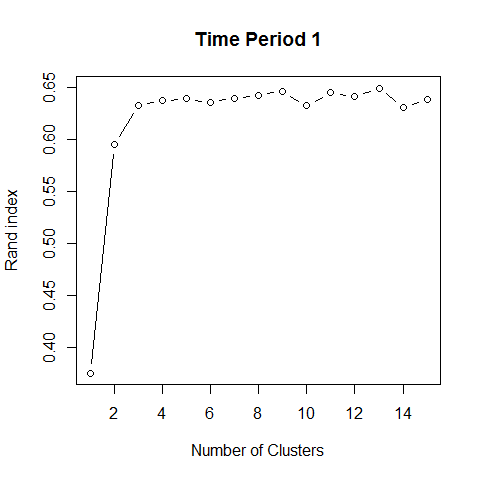
\includegraphics[width=0.32\textwidth]{images/chapter4/elbowMemberShipAgreement1.png}
                     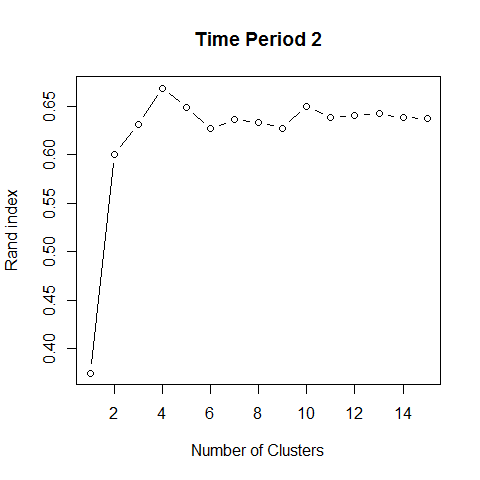
\includegraphics[width=0.32\textwidth]{images/chapter4/elbowMemberShipAgreement2.png}
                     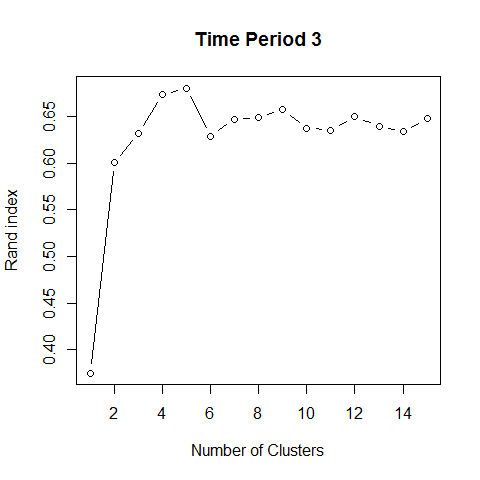
\includegraphics[width=0.32\textwidth]{images/chapter4/elbowMemberShipAgreement3.png}
                 }\\
                 \subfigure{
                     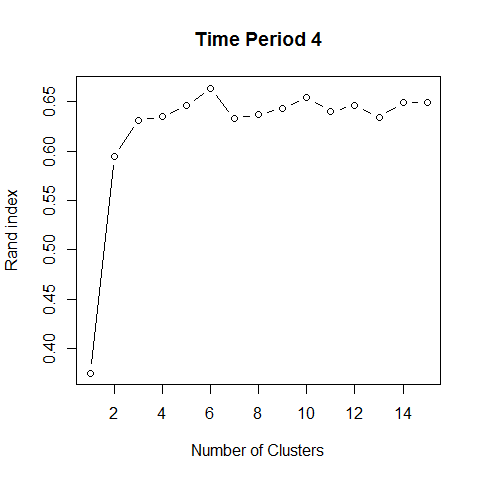
\includegraphics[width=0.32\textwidth]{images/chapter4/elbowMemberShipAgreement4.png}
                     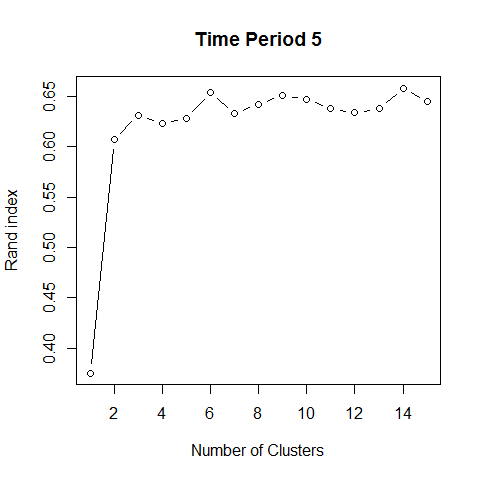
\includegraphics[width=0.32\textwidth]{images/chapter4/elbowMemberShipAgreement5.png}
                     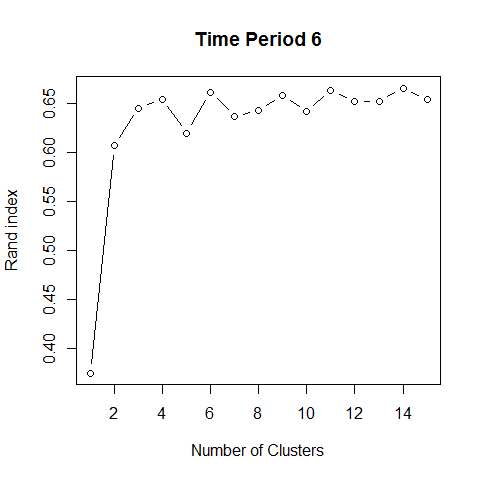
\includegraphics[width=0.32\textwidth]{images/chapter4/elbowMemberShipAgreement6.png}    
                 }\\
                 \subfigure{
                     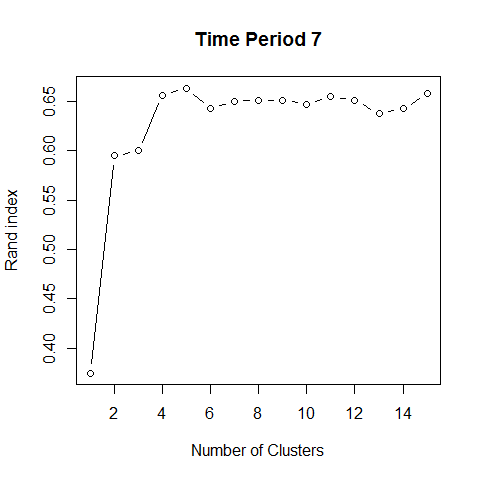
\includegraphics[width=0.32\textwidth]{images/chapter4/elbowMemberShipAgreement7.png}
                     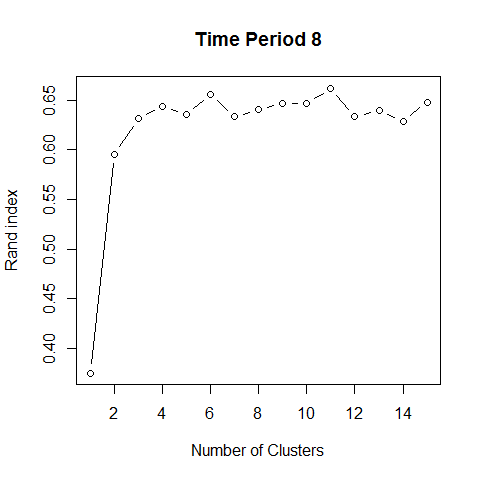
\includegraphics[width=0.32\textwidth]{images/chapter4/elbowMemberShipAgreement8.png}
                     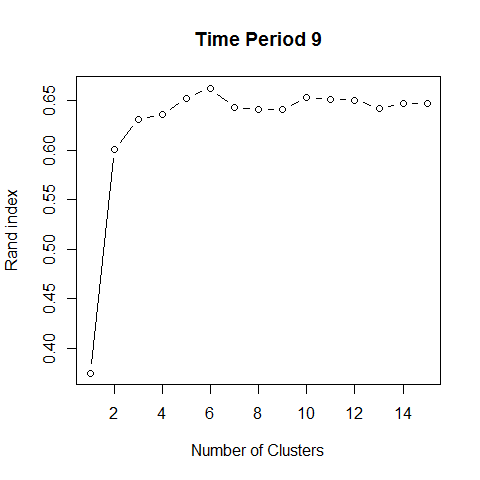
\includegraphics[width=0.32\textwidth]{images/chapter4/elbowMemberShipAgreement9.png}    
                 }\\
             \end{minipage}}
             \caption{Using rand index to find the best member ship matches between clusters and classes.}
             \label{fig:elbowMemberShipAgreement}
         \end{figure}
         
 The synthetic data set is created with distinct four clusters, so its results can be comparable with the results of the public goods game data sets.
         
\subsection{Choosing External Cluster Validity Indices}
\label{sec:ChoosingExternalClusterValidityIndices}
         
As explained in the methodology section of chapter three, we propose using external cluster validity indices and area under the curve AUC to measure the changes which might occur in the behaviour of the items between multiple time points in a temporal data. Many external cluster validity indices are available \cite{Arbelaitz2012} to measure the validity of clusters produced by clustering methods compared with the natural partitions that exist. In chapter 17 of their book, Zaki et al. \cite{Zaki2014} categorised the external clustering validities into three types: matching based measures, entropy-based measures and pairwise measures. For more information on external cluster validity indices, please refer to chapter two.
         
As is the case for matching-based measures,  external cluster validity indices calculate the match of the clusters to the partitions. This means this measure is not concerned about individual element differences between clusters and partition.  This category might, therefore,  not be beneficial in calculating the changes over time.
         
The second category of external cluster validity indices, entropy-based measures, calculates the difference of entropy between clusters and ground truth partitions. This method is not concerned about individual items in the clusters and partitions. However, we used one measure of this category, Variation of Information VI, because the entropy of the clusters might be affected by the change of items within the clusters. We also used VI for comparison purposes with other indices.
         
The last category, pairwise measures, measures cluster validity by comparing the produced clusters and original labels of items' classes. As this category calculates the validity using all elements of the data set,  it may, therefore, be the most appropriate category to calculate the items' changes over time points. Three instances of pairwise measures are used in this chapter: the Jaccard Coefficient, Rand Statistic and the Fowlkes-Mallows Measure. Please refer to chapter two for more details on each of these measures.
         
Standard criteria for different external cluster validity indices must be maintained so that the final result which quantifies the amount of change in each time point reflects the actual change in the groups' items regardless of the measure used. To ensure the measures are standard, they should follow two rules (1) the scale of the measure should be between 0 and 1 (2) with 0 being the total change and 1 the perfect match between any time point and reference of behaviour. However, not all measures follow these rules. For example, in the selected measures the VI is not bound to any scale, and zero is considered as a perfect match. Thus, the results of this measure should be (1) scaled to the range of  [0-1] (2) then reversed, by subtracting the current time points' result from the maximum change which can be obtained from the data set.
         
\subsection{Using Internal Cluster Validity Indices}
         
We have considered using internal cluster Validity Indices alongside external cluster validity indices.  We tested multiple internal cluster validity indices such as Davies Bouldin index \cite{Davies1979a}, and Dunn index \cite{Dunn1973a}. However, all internal cluster validity indices are designed to measure the validity of the clusters using an \gls{ItemsAgglomeration} in the clusters and distances among clusters. This means that the Internal cluster validity indices can detect changes which are happening to the clusters in general but not the individual changes in items. We, therefore, dismissed the results produced by this method.
         
\subsection{Using Area Under the Curve}

 As explained by Fawcett \cite{Fawcett2006}, AUC calculates the area under the Receiver Operating Characteristic ROC curve and is plotted as a relationship between true positive rate and false positive rate. As this criterion uses an element-wise comparison to find the number of true positive and false positives, this measure might be useful in calculating the changes between two time points. Originally, this measure was used to demonstrate the quality of binary classification. However, a generalised method of multiple classes is presented by Hand et al. \cite{Hand2001}. Please refer to chapter two for more details on AUC.
         
AUC is designed to measure how well a classifier performs in predicting classes of elements compared with the true labels of the elements. This means, unlike pairwise external cluster validity measures, before using AUC to measure the change over time, the cluster labels of time points should be matched. There are a number of methods to match clusters \cite{Rezaei2016,Halkidi2002a}. We have used these methods:
         
\begin{itemize}
    \item Using the cluster centroids of n time point to be the suggested start centroid for the n+1 time point. However, this method only works with k--means and PAM, but it is not an option for hierarchical clustering.
    \item Using distances between centroids of the produced clusters in both time points as a reference for matching between clusters.
    \item Comparing the elements' membership in clusters between these two time points to find the matches between clusters.
\end{itemize}
         
 \subsection{Different Reference of Behaviours for Items}
 \label{sec:DifferentReferenceofBehavioursforItems}
         
This study considers three different references of behaviours.  However, in this chapter,  we will test two. They are  1) the first time point is used as a reference of behaviour for all other time points 2) The previous time point is used to be the reference of behaviour for the current time point. In the next chapter, a new classification method will be proposed to classify items in temporal data sets. This classification will be used as a reference of the items' behaviour in chapter six.
         
Each of these different references of behaviour brings different meaning and can be used in various ways. The first time point can be used as a reference of behaviour to quantify the progress of change which happens to the items in any later time points in the data set. An example of that is if we want to quantify the change of behaviour of players in PGG from the first round of the game to any round of the game.     Using the previous time point as a reference for the current time point means we aim to stepwise measure changes in items' behaviour between any time point. This can be used to measure the stability of change over time. An example of using this method is when we want to check the stability of changes that can occur in player behaviour between time points. Items' classes such as reference of behaviour can be used to quantify items' deviation from their own generalised behaviour at any time point.
         
         
         
 \section{Testing the Proposed Method}
         
We conducted this experiment to show that the proposed method can be used for measuring changes among various groups over time in temporal data. The synthetic data is created so that obvious changes of behaviour can be observed by introducing jumps for items from one group to another. The item set contains 500 items grouped into four distinct groups. The data is mutated repeatedly using jumps and jiggles 19 times to create 20 time points (the original data set is the first one). To illustrate the original and mutated data three time points are shown in Figure \ref{fig:synthesisData2}. Please refer to section \ref{CreatingaSyntheticData} in chapter three for a detailed explanation of the method of creating the data set.
         
\begin{figure}[!h]
\centering
{
    \subfigure[First time point]{
        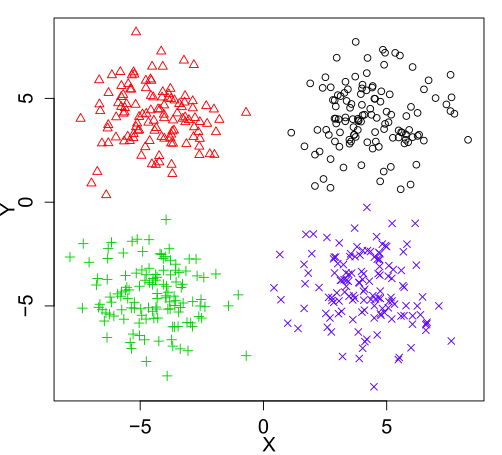
\includegraphics[width=0.31\textwidth]{images/chapter3/synthesisDataFirst.png}\label{fig:synthesisData_first2}}
    \subfigure[Middle time point]{
        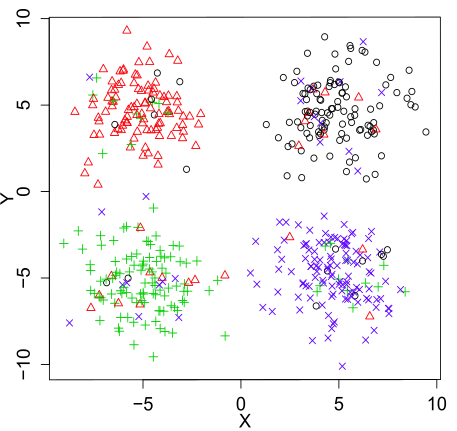
\includegraphics[width=0.30\textwidth]{images/chapter3/synthesisDataMid.png}\label{fig:synthesisData_mid2}}
    \subfigure[Last time point]{
        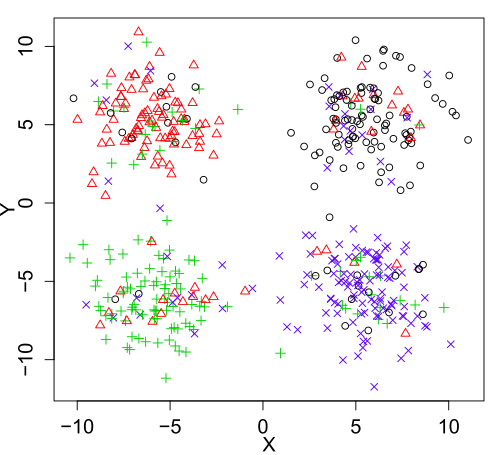
\includegraphics[width=0.30\textwidth]{images/chapter3/synthesisDataLast.png}\label{fig:synthesisData_last2}}}
\caption{Three time points (first, middle and last) from the 20 time points created overall. The first time point, contains 500 items and separated into four clusters, is the original data set other time points are created by mutating (jumping) items of four clusters from one cluster into another.}
\label{fig:synthesisData2}
\end{figure}
         
To test Hypothesis \ref{hypo:diffCluster}, multiple clustering methods are used in this experiment to group items in each time point of the synthetic data set. The clustering methods are chosen based on the criteria discussed in section \ref{sec:ChoosingClusteringAlgorithms}. Moreover to test Hypothesis \ref{hypo:diffCVI}, multiple external cluster validity indices and the AUC of ROC are used to measure the magnitude of changes happening to the items in the produced groups using different clustering methods. The choice of external cluster validity indices are based on the prior discussion in section \ref {sec:ChoosingExternalClusterValidityIndices}. We also tested the two types of reference of behaviour for items. To do so, all tests are run twice. The first occasion considered the first time point as the reference of behaviour and then all time points were compared with it. The second time considered previous time point as the reference of behaviour for the current time point. Please refer to section \ref{sec:DifferentReferenceofBehavioursforItems} for more details.

Using this method, both clustering techniques, external cluster validity indices, and reference of behaviour, produce a result of an array of values which quantify the difference between each time point and the reference of behaviour. These values can be reported as a list of values, or a table. However, to obtain an idea of the degree of change of items of groups through time points, an x,y chart can be used with time points as x-axes and the magnitude of change values scaling from 0 to 1 as y-axes. Figure \ref{fig:test_ChangeMeasuers_Firs} shows results of k--means, PAM, c--means and hierarchical clustering methods using the first time point as the reference of behaviour to calculate the magnitude of changes which happen to the groups of items in consequent time points in the test data set. The amount of change is measured by using different external cluster validity indices and AUC of ROC. Moreover, Figure \ref{fig:test_ChangeMeasuers_Cons} shows results for the proposed method using the same clustering techniques and external cluster validity indices although it uses the previous time point as the reference of behaviour for the current one.

Figure \ref{fig:test_ChangeMeasuers_Firs} shows a gradual shift from the first time point as each new time point introduces further mutations for the data set and, hence, further drifting from the original location of the items. While all measures confirm the gradual change of progressing time points, however, not all of them react in the same way. The major noticeable difference is that FM and Jaccard are overreacting to the changes and show high sensitivity to it. As the VI values are scaled and flipped, they correspond to fit the rules laid out in section  \ref{sec:ChoosingExternalClusterValidityIndices}. Results are, therefore, shown in a very saturated scale as the lowest point become zero due to the scaling and flipping. However, the actual changes are a small percentage of the overall items suggesting that these scales of change by the two measures could be due to the original design of these two measures to show the difference between clusterings and real classes. Moreover, all results of the hierarchical clustering show a slightly different change pattern than other clustering methods. Another noticeable result is that k means clustering shows an increased sensitivity to the changes between 14 and 15 time points. The same sensitivity is not depicted by other clustering algorithms.
         
\begin{figure}[!h]
\hfill{\begin{minipage}{\dimexpr \textwidth-2\fboxsep-2\fboxrule}% maximum allowed
        \centering
        \subfigure[K--means Clustering]{
            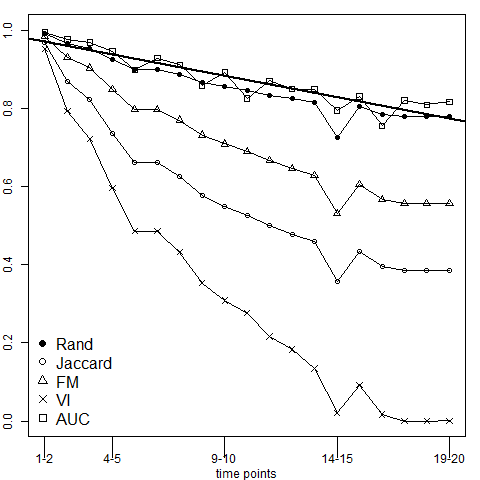
\includegraphics[width=0.45\textwidth]{images/chapter4/test_kmeansClusters_Firs.png}
        }
        \subfigure[PAM Clustering]{
            \includegraphics[width=0.45\textwidth]{images/chapter4/test_PAMClusters_Firs.png}
        }\\
        
        \centering
        \subfigure[C--means Clustering]{
            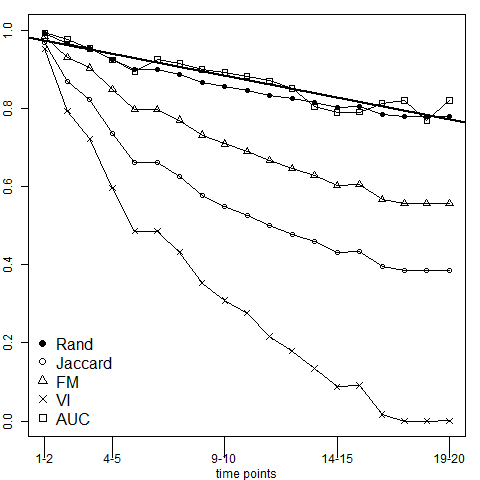
\includegraphics[width=0.45\textwidth]{images/chapter4/test_cmeansClusters_Firs.png}
        }
        \subfigure[Hierarchical Clustering]{
            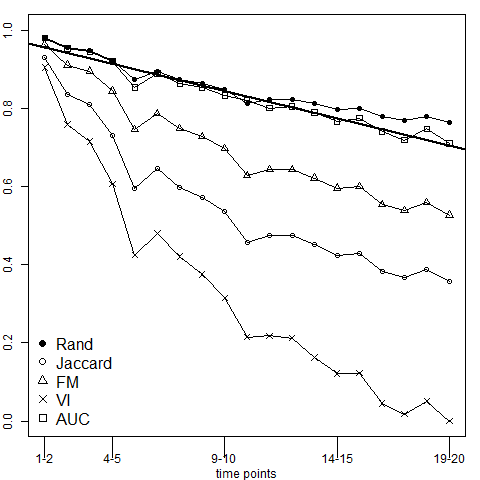
\includegraphics[width=0.45\textwidth]{images/chapter4/test_hierClusters_Firs.png}
        }\\
        
    \end{minipage}}
    \caption{Results of various clustering methods using the first time point as a reference of behaviour to calculate the magnitude of changes which happen to the groups of items in consequent time points in the test data set. The amount of change  is measured by using different external cluster validity indices and AUC of ROC.}
    \label{fig:test_ChangeMeasuers_Firs}
\end{figure}
             
             
Figure \ref{fig:test_ChangeMeasuers_Cons} shows the difference between any two consequent time points. PAM and c--means clustering methods created visually similar results while k--means and hierarchical clustering produced very different results. While all clustering methods are producing a greater change between time points 13-15,  k--means, however,  shows an extreme change in the same time periods. In these results, VI shows exaggerated differences between time points. However, FM and Jaccard results display the difference between time points more than AUC and Rand. AUC and Rand results might reflect the reality of the changes, but the changes become unnoticeable due to the small scaling.
             
\begin{figure}[!h]
\hfill{\begin{minipage}{\dimexpr \textwidth-2\fboxsep-2\fboxrule}% maximum allowed
        \centering
        \subfigure[K--means Clustering]{
            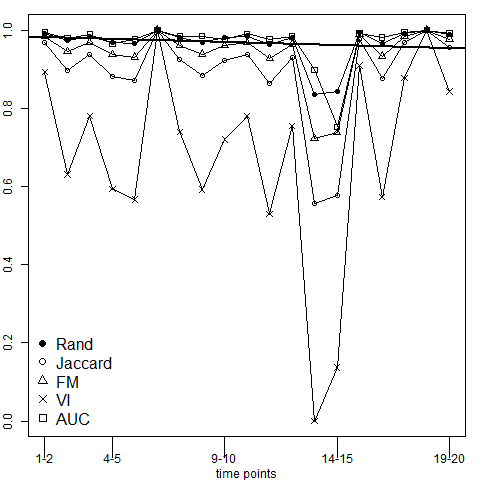
\includegraphics[width=0.45\textwidth]{images/chapter4/test_kmeansClusters_Cons.png}
        }
        \subfigure[PAM Clustering]{
            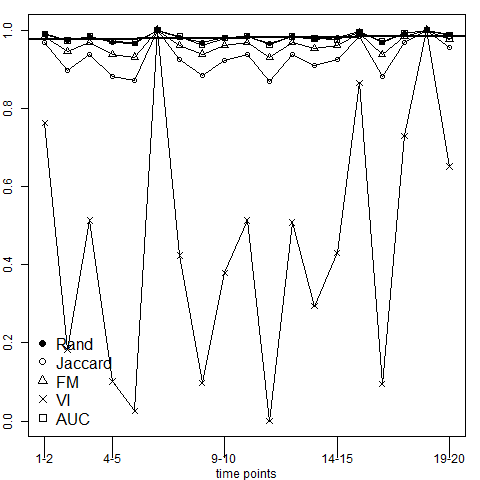
\includegraphics[width=0.45\textwidth]{images/chapter4/test_pamClusters_Cons.png}
        }\\
        
        \centering
        \subfigure[C--means Clustering]{
            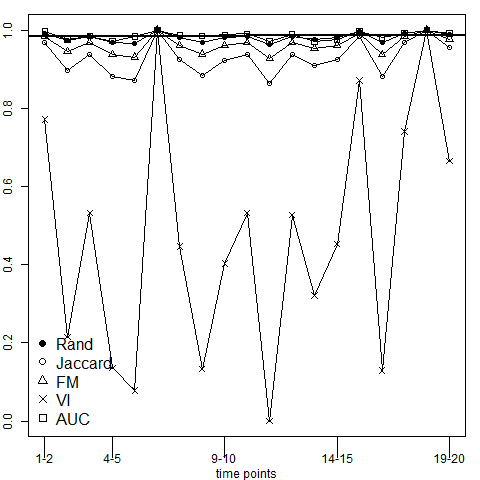
\includegraphics[width=0.45\textwidth]{images/chapter4/test_cmeansClusters_Cons.png}
        }
        \subfigure[Hierarchical Clustering]{
            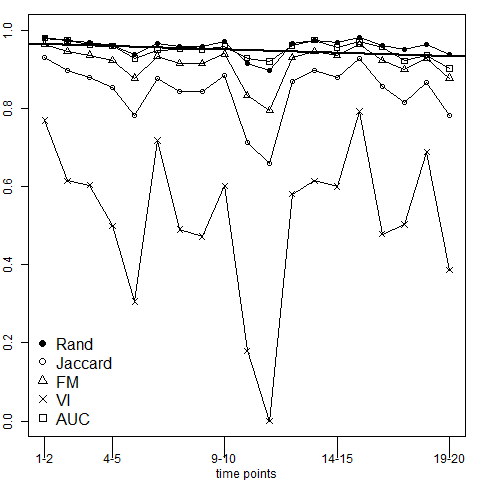
\includegraphics[width=0.45\textwidth]{images/chapter4/test_hierClusters_Cons.png}
        }\\
        
    \end{minipage}}
    \caption{Results of various clustering methods using the previous time point as reference of behaviour to calculate the magnitude of changes which happen to the groups of items in consequent time points in the test data set.}
    \label{fig:test_ChangeMeasuers_Cons}
\end{figure}
                 
                 
                 
The Friedman test is used to validate Hypothesis \ref{hypo:diffCluster} on the proposed method for measuring changes over time using acquired results from the synthetic data set. The p.value of the four samples for measuring changes of time points against the original data set is 4.947325e-14 and p.value for measuring changes of current time points against the previous time point is 1.895672e-14. This means, in both cases, we can not reject the null hypothesis, and hence, the samples are different. However, a closer look at the results by comparing every two samples of different clustering methods using Wilcoxon tests reveals (see Table \ref{tab:Cluster_Pvalue_Test}) that all p.values are higher than 0.05 for the samples used the first time point as the reference of behaviour. For those samples which using previous time point as the reference of behaviour, only hierarchical clustering produced p.values less than 0.05 when compared with other samples. This means all three clustering methods are producing the same results for measuring changes over time. Given that, we can consider Hypothesis \ref{hypo:diffCluster}  to hold true especially given all clustering methods are confirming that the items inside the groups are changing gradually over time. The difference is only in the sensitivity to the change, an aspect of the clustering method.

\begin{table}[!h]
    \ra{1.3}
    \small
    \centering
    \caption{ P-values of Wilcoxon-test for each pair of clusters.}
    \label{tab:Cluster_Pvalue_Test}
    \begin{tabular}{llll}
        \toprule
        \textbf{Clustering1} & \textbf{Clustering2}  & \textbf{p-Value First} & \textbf{p-Value Consequent} \\ \midrule
        k--means      & c--means       & 0.9778971     & 0.6262925          \\ 
        k--means      & PAM          & 0.7868127     & 0.8050843          \\ 
        k--means      & hierarchical & 0.5369699     & 0.000704285        \\ 
        c--means      & PAM          & 0.7555338     & 0.7776328          \\ 
        c--means      & hierarchical & 0.4877342     & 3.17E-05           \\ 
        PAM         & hierarchical & 0.6903287     & 4.68E-05           \\ 
        \bottomrule
    \end{tabular}
\end{table}


To validate Hypothesis \ref{hypo:diffCVI}, the similarity of result samples produced by different external cluster validity indices have to be measured. We used the Friedman test to check if all the results are similar to the null hypothesis that assumes similarity for the produced results in measuring the amount of change for all time points using different external cluster validity indices or AUC. Two p-values are produced. The first p-value = 5.232651e-44 for the samples which are produced by measuring the behaviour of each time point compared to the first time point. The second p-value = 1.416841e-53 for the results which are produced by comparing each time point with its successor.  In both cases, p-values are smaller than 0.05.  The null hypotheses should, therefore, be rejected as the samples are different.  Moreover, we conducted a Wilcoxon test on the samples to take a closer look at the results of every pair of two samples produced with different measures. As shown in Table  \ref{tab:ECVI_Failed_Pvalue_Test}, the p-values (except for the AUC and Rand pair) are smaller than 0.05 which indicates that these pairs are different from each other. This means that different measures are producing significantly different results. Hence, Hypothesis \ref{hypo:diffCVI} can not be true. So, further examination of the results is required to check whether the proposed method can be used to measure changes over time or not.

However, despite the measures producing different results, as proved by using different statistical tests, we can see from figures \ref{fig:test_ChangeMeasuers_Firs} and \ref{fig:test_ChangeMeasuers_Cons} that all measures indicate the gradual change in the data with different sensitivities to the amount of change. As the data is synthesised and new time points are created by mutating the current time point, we can, thus, confirm that the results reflect the gradual change which already exists in the data. Therefore, the difference between samples might be a direct result of the different sensitivities which each measure is created for, and included in its method of calculating differences in group similarities between predicted results and true labels of the items.

Measures with different sensitivities proved to be a positive aspect of the proposed method for measuring changes over time in various situations as it enables us to control the amount of sensitivity needed for a specific situation or application. For example in Figure \ref{fig:test_ChangeMeasuers_Firs}, Rand and AUC measures reflect the amount of change well, while in Figure \ref{fig:test_ChangeMeasuers_Cons} Jaccard and FM can highlight changes which can not be detected by the previous two measures.



\begin{table}[!h]
    \ra{1.3}
    \small
    \centering
    \caption{P-values of Wilcoxon-test for each pair of external cluster validity indices and AUC.}
    \label{tab:ECVI_Failed_Pvalue_Test}
    \begin{tabular}{llll}
        \toprule
        \textbf{Clustering1} & \textbf{Clustering2}  & \textbf{p-Value First} & \textbf{p-Value Consequent} \\ \midrule
        Rand      & Jaccard  & 1.947533e-17     & 2.182083e-13          \\ 
        Rand      & FM       & 1.857682e-11     & 4.051658e-07          \\ 
        Rand      & VI       & 4.131331e-13     & 9.372113e-24          \\ 
        Rand      & AUC      & 0.9251302        & 0.5177034             \\ 
        
        Jaccard   & FM       & 3.865308e-08     & 3.565382e-06          \\ 
        Jaccard   & VI       & 1.977779e-18     & 1.242547e-22          \\ 
        Jaccard   & AUC      & 1.103106e-17     & 2.012194e-13          \\ 
        
        FM        & VI       & 1.956715e-15     & 3.196178e-23          \\ 
        FM        & AUC      & 2.114171e-11     & 1.110287e-06          \\ 
        
        VI        & AUC      & 3.718286e-13     & 1.051501e-23          \\     
        \bottomrule
    \end{tabular}
\end{table}

To be able to use the proposed method for measuring changes over time in temporal data, it should, at least, be proven that each measure independently from other measures can produce consistent results for different clustering methods. Another test is conducted to check if a measure can produce consistent results across multiple clustering methods. The results for each measure produced by different clustering algorithms are compared, and the p-value for the Wilcoxon test is produced as shown in Table \ref{tab:ECVI_Pvalue_Test}. P-values of each pair of the produced samples are higher than 0.05 except for hierarchical clustering when using previous time point as a reference of behaviour (consequent test). This means we can not reject the null hypothesis because the results of measures are consistent across multiple clustering methods. That the p-value is not smaller than 0.05 in hierarchical clustering might be because hierarchical clustering itself produces different groups than other clustering methods as has been previously proven in this section.


\begin{table}[!h]
    \ra{1.3}
    \small
    \centering
    \caption{P-values of Wilcoxon-test for each pair of external cluster validity indices or AUC.}
    \label{tab:ECVI_Pvalue_Test}
    \begin{tabular}{rllllll} \toprule
        Cluster1  & Cluster2   & Rand        & Jaccard     & FM          & VI          & AUC        \\ \midrule
        \multicolumn{1}{l}{\textbf{First}}       \\        
        k--means       & c--means        & 0.930085   & 0.930085   & 0.930085   & 1           & 0.941807  \\
        k--means       & PAM           & 0.883816   & 0.906934   & 0.906934   & 0.906934    & 0.165448  \\
        k--means       & hierar           & 0.704262   & 0.704262   & 0.682708   & 0.704262    & 0.085021  \\
        c--means       & PAM           & 0.965026   & 0.988339   & 0.988339   & 0.91851     & 0.188877  \\
        c--means       & hierar           & 0.579058   & 0.579058   & 0.579058   & 0.682708    & 0.08502   \\
        PAM          & hierar           & 0.579058   & 0.579058   & 0.579058   & 0.682708    & 0.539772  \\
        \multicolumn{1}{l}{\textbf{Consequent}}\\        
        k--means       & c--means        & 0.558817   & 0.558817   & 0.558817   & 0.619407    & 0.609161  \\
        k--means       & PAM           & 0.529826   & 0.539462   & 0.539462   & 0.640234    & 0.578892  \\
        k--means       & hierar           & 0.00319    & 0.003505   & 0.003504   & 0.018246    & 9.14E-05  \\
        c--means       & PAM           & 0.976681   & 0.98834    & 0.98834    & 0.98834     & 0.214412  \\
        c--means       & hierar          & 6.34E-05   & 6.34E-05   & 6.34E-05   & 0.000787    & 8.05E-07  \\
        PAM          & hierar          & 4.94E-05   & 4.94E-05   & 4.94E-05   & 0.001192    & 6.92E-06  \\
        
        \bottomrule
    \end{tabular}
\end{table}

In this section, we demonstrated and proved that using different clustering techniques will produce similar results for measuring changes over time. We also proved that using the same measure (that is external cluster validity indices or AUC of ROC) produces consistent results across all clustering methods. This is an indication that the proposed method can be used to measure changes over time and produce a single value which indicates the amount of change that happens to items' membership in the available groups at different time points.


\section{Measuring Players' Strategy Change over Time}
The main objective of this experiment is to quantify how players' change in strategy in the public goods game can contribute to the understanding of the players' behaviour and present a tool for economists to measure the amount of change for different set-ups of their experiment. Another objective of this experiment is to demonstrate the ability of the proposed method to produce quantifiable measures for changes in items. In the temporal data and provide interpretable results. We compare the results and findings of our method with the MONIC method which is originally used to measure cluster changes in a data stream  \cite{Spiliopoulou2006}.

In section \ref{PublicGoodsGamesData} of chapter three, two data sets of PGG are introduced. For this experiment,  both data sets are used to measure players behaviour and strategy change during the consequent rounds of the game. The attribute of players own contribution and their expectation of other players' contribution at each time point are used by this method to find the magnitude of the change. These two data sets have different groups of players and different lengths as the first data set is 10 rounds length and the second is 27. Therefore, these two data sets are used separately and treated as different data sets in this experiment. Based on the previous discussion in section \ref{sec:Choosing-Number-of-Clusters}, we used four clusters to cluster players in each time point using k--means, PAM, c--means and hierarchical clustering methods.These methods were selected based on our discussion in section \ref{sec:ChoosingClusteringAlgorithms}.

As both data sets of PGG share the same experiment settings and setup, it can be hypothesised that the results of the behaviour change should be consistent with regards to the length of the experiment which, in turn,  might affect the behaviour of players \cite{Figuieres2010}. While we use all previously selected external cluster validity indices as in section \ref{sec:ChoosingExternalClusterValidityIndices} and AUC of ROC. We will, however, depend on AUC and Rand results to compare the behaviour of players in these two different data sets as we demonstrated that these two measures produce more consistent results than the rest of the measures.


\subsection{Using Proposed Method}

Prior to the analysis of the players' behaviour, we checked both Hypothesis \ref{hypo:diffCluster} and \ref{hypo:diffCVI} using real data sets. Using p-value, as described in the previous section, similarities between results of different clustering and external cluster validity indices are tested. P-value results are shown in Appendix \ref{App:P-Values-for-Public-Goods-Game}. While slightly different results are produced especially for 27 period data set, the results are consistent with the results of synthetic data. This can be considered as additional evidence that the presented method for measuring changes over time can be used with real data sets.

Different types of reference point reveal different aspects of players' strategy change. By using the first time point as the reference of behaviour, we can detect drift of players' behaviour from the initial expectation and contribution. As shown in Figure \ref{fig:game10_ChangeMeasuers_Firs} for 10 rounds data set and Figure \ref{fig:game27_ChangeMeasuers_Firs} for 27 rounds, players in both data sets are gradually drifting away from their initial game plan and expectation. This trend can be seen with all four clustering methods with the different measurement methods of external cluster validity indices and AUC. Because the results of AUC and Rand are consistent across all clustering methods, we used AUC to calculate the linear regression of the results. The negative results of linear regression is an indication that players increase their behaviour of drifting away from their original gameplay.

By using the previous time point as the reference of behaviour, we can measure the amount of change between any two consecutive time points. This allows detection of players' behaviour transition from one time point to another. Figure \ref{fig:game10_ChangeMeasuers_Cons} of the 10 rounds data set shows that players strategy change from one time point to another is constant. This is indicated by the linear regression of AUC and Rand measures. In contrast Figure \ref{fig:game27_ChangeMeasuers_Cons} of 27 rounds shows that the change between time points is decreasing throughout the progress of the game. 

At first glance, the results of 10 and 27 rounds data sets are not consistent. However, after taking a closer look at the results, we can detect that the players' behaviour change in 27 rounds data set is stable without any decrease until round 10 of the game. As shown in Figure \ref{fig:contributionRound27} this decrease might be due to the fact that most of the players dropped their contribution to zero when they reached round 10. This means there is no room for further change left in the game except some players randomly start to increase their contribution again but the rise is not constant, so after round 10 we detect less change than expected.

\begin{figure}[!h]
\hfill{\begin{minipage}{\dimexpr \textwidth-2\fboxsep-2\fboxrule}% maximum allowed
    \centering
    \subfigure[K--means Clustering]{
        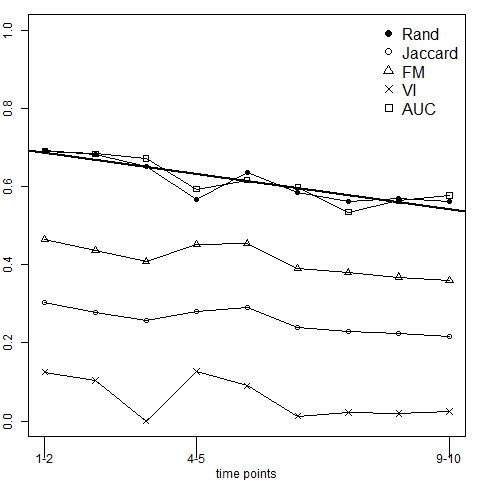
\includegraphics[width=0.45\textwidth]{images/chapter4/game10_kmeansClusters_Firs.png}
    }
    \subfigure[PAM Clustering]{
        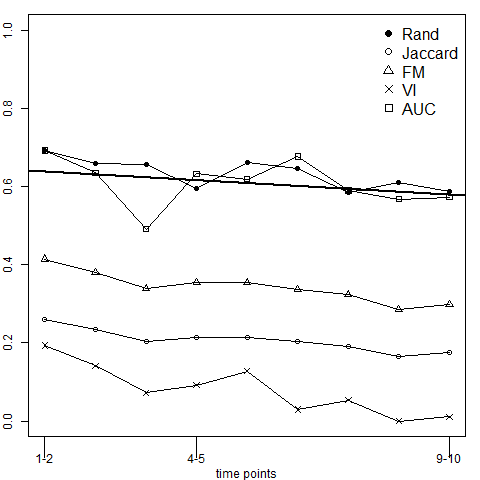
\includegraphics[width=0.45\textwidth]{images/chapter4/game10_pamClusters_Firs.png}
    }\\
    
    \centering
    \subfigure[C--means Clustering]{
        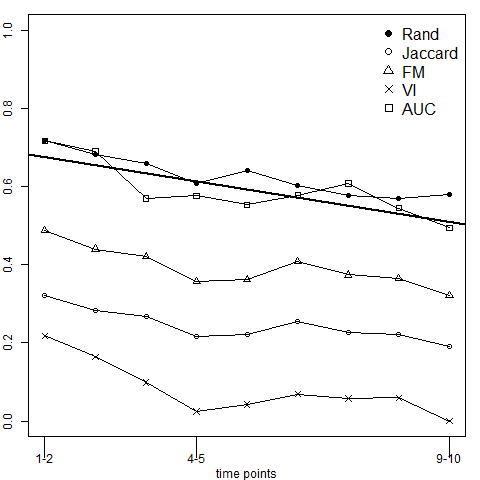
\includegraphics[width=0.45\textwidth]{images/chapter4/game10_cmeansClusters_Firs.png}
    }
    \subfigure[Hirarchical Clustering]{
        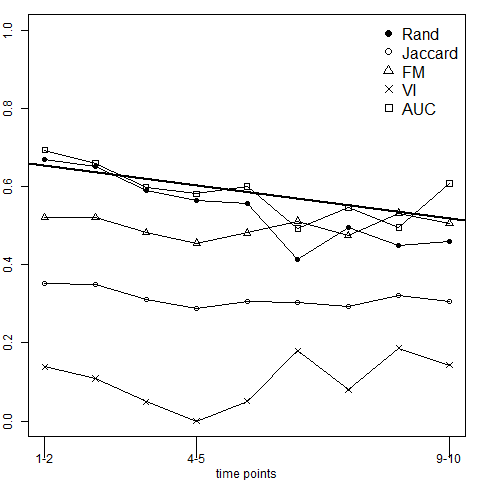
\includegraphics[width=0.45\textwidth]{images/chapter4/game10_hierClusters_Firs.png}
    }\\
    
\end{minipage}}
\caption{Results of various clustering methods using the first time point as reference of behaviour to calculate the magnitude of changes which happen to the groups of items in consequent time points in the 10 rounds PGG data set.}
\label{fig:game10_ChangeMeasuers_Firs}
\end{figure}
    
    
    
\begin{figure}[!h]
\hfill{\begin{minipage}{\dimexpr \textwidth-2\fboxsep-2\fboxrule}% maximum allowed
        \centering
        \subfigure[K--means Clustering]{
            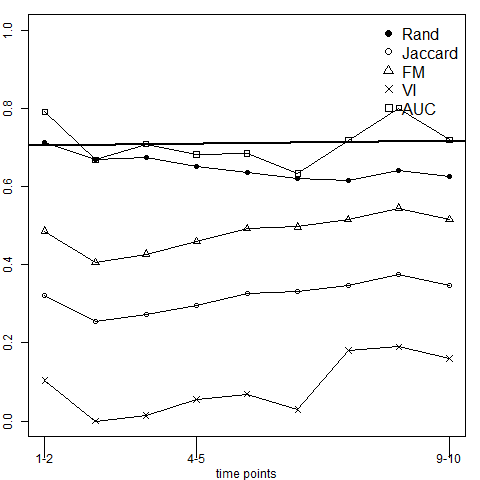
\includegraphics[width=0.45\textwidth]{images/chapter4/game10_kmeansClusters_Cons.png}
        }
        \subfigure[PAM Clustering]{
            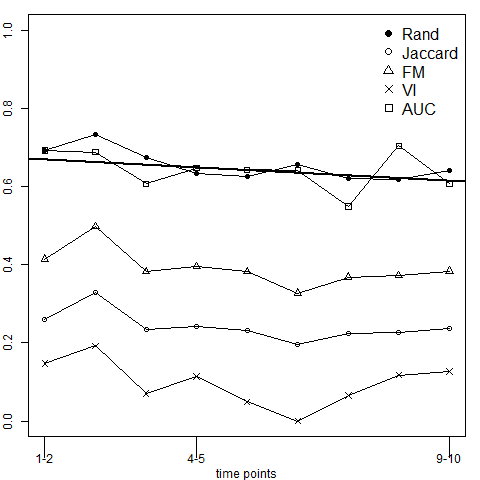
\includegraphics[width=0.45\textwidth]{images/chapter4/game10_pamClusters_Cons.png}
        }\\
        
        \centering
        \subfigure[C--means Clustering]{
            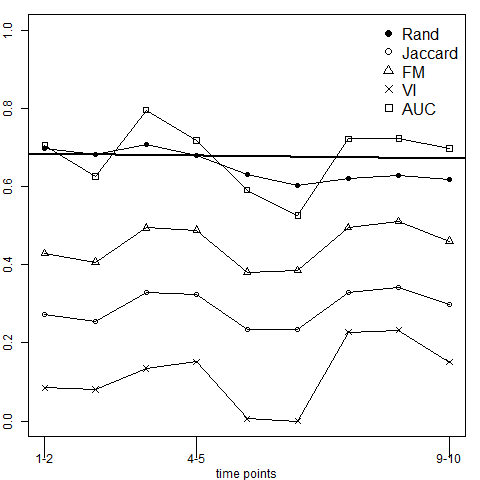
\includegraphics[width=0.45\textwidth]{images/chapter4/game10_cmeansClusters_Cons.png}
        }
        \subfigure[Hirarchical Clustering]{
            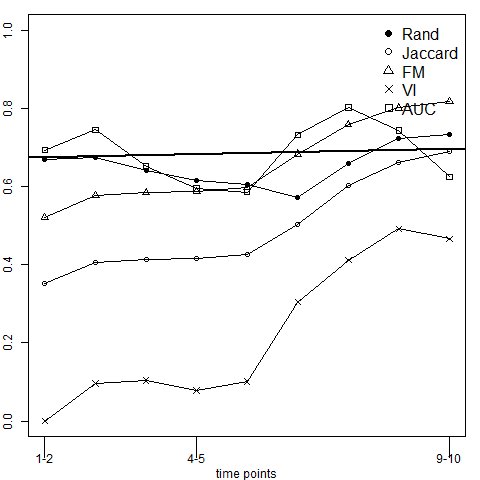
\includegraphics[width=0.45\textwidth]{images/chapter4/game10_hierClusters_Cons.png}
        }\\
        
    \end{minipage}}
    \caption{Results of various clustering methods using the previous time point as reference of behaviour to calculate the magnitude of changes which happen to the groups of items in consequent time points in the 10 rounds PGG data set.}
    \label{fig:game10_ChangeMeasuers_Cons}
\end{figure}
        
        
As we hypothesised in the previous section, player behaviour has to be consistent in both data sets. The results for measuring changes using the first time point as the reference of behaviour are compatible as players' contribution drops gradually in both cases. The results of using the previous time point as the reference of behaviour show that players strategy change is constant until round 10. In 27 rounds data set, most players' contribution after round 10 dropped to zero meaning there is no room for further change in their strategy. Hence, the amount of change in their strategy decreases and their game pattern starts to become similar between any two consequent time points. These results show that the proposed hypothesis holds true. This is yet another indication that the proposed method produces consistent results for similar situations.


\begin{figure}[!h]
\hfill{\begin{minipage}{\dimexpr \textwidth-2\fboxsep-2\fboxrule}% maximum allowed
        \centering
        \subfigure[K--means Clustering]{
            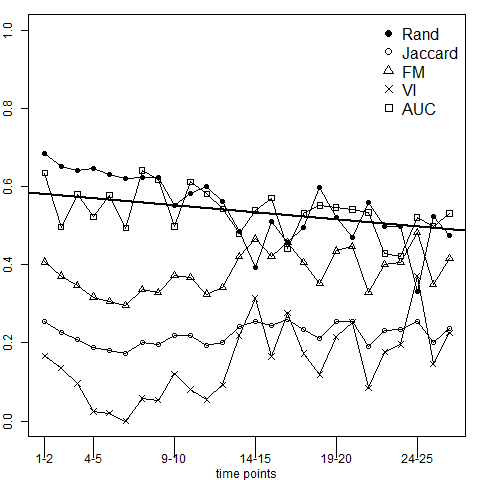
\includegraphics[width=0.45\textwidth]{images/chapter4/game27_kmeansClusters_Firs.png}
        }
        \subfigure[PAM Clustering]{
            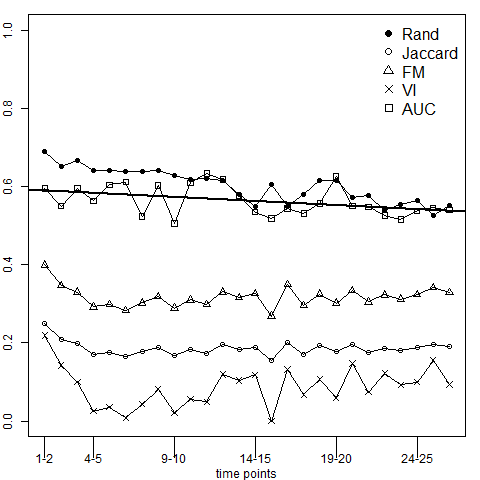
\includegraphics[width=0.45\textwidth]{images/chapter4/game27_pamClusters_Firs.png}
        }\\
        
        \centering
        \subfigure[C--means Clustering]{
            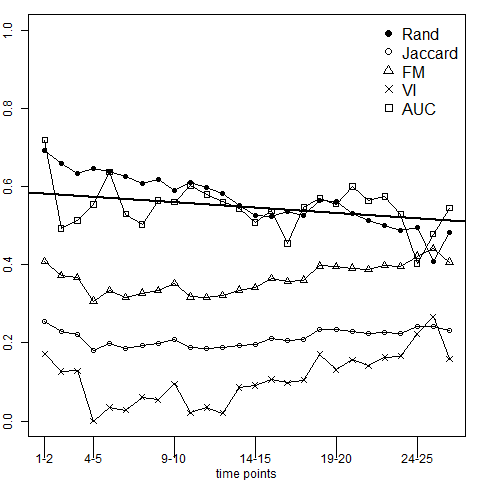
\includegraphics[width=0.45\textwidth]{images/chapter4/game27_cmeansClusters_Firs.png}
        }
        \subfigure[Hirarchical Clustering]{
            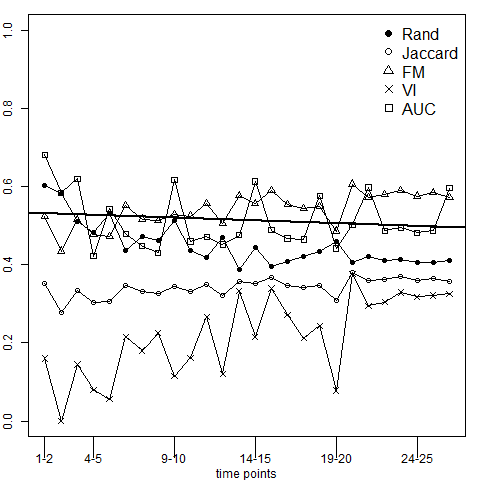
\includegraphics[width=0.45\textwidth]{images/chapter4/game27_hierClusters_Firs.png}
        }\\
        
    \end{minipage}}
    \caption{Results of various clustering methods using the first time point as reference of behaviour to calculate the magnitude of changes which happen to the groups of items in consequent time points in the 27 rounds PGG data set.}
    \label{fig:game27_ChangeMeasuers_Firs}
\end{figure}
            
            
The results of the proposed method for both data sets are compatible with the findings of economists \cite{Fischbacher2010,Hoice2008,Chaudhuri2006}. However, this method provides a tool which enables them to quantify changes in players behaviour. Quantifying behaviour change is important so they can measure the nuanced differences between various gameplay setups like the length of the rounds, the percentage of the rewards from the public project, and knowing the identity of other players.




\begin{figure}[!h]
\hfill{\begin{minipage}{\dimexpr \textwidth-2\fboxsep-2\fboxrule}% maximum allowed
        \centering
        \subfigure[K--means Clustering]{
            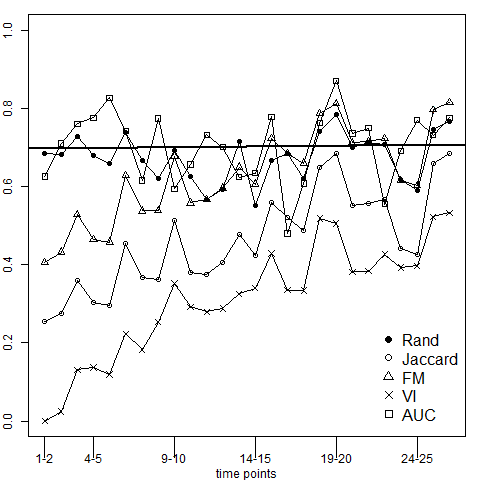
\includegraphics[width=0.45\textwidth]{images/chapter4/game27_kmeansClusters_Cons.png}
        }
        \subfigure[PAM Clustering]{
            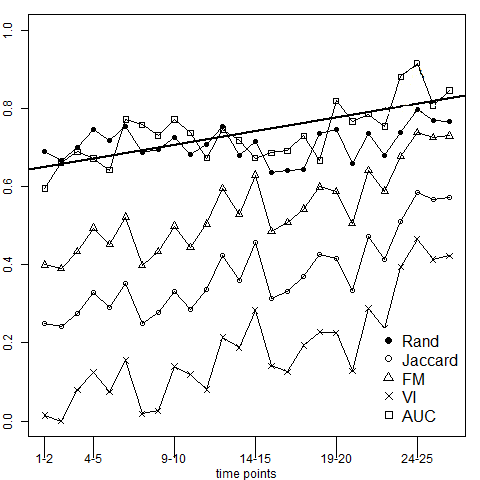
\includegraphics[width=0.45\textwidth]{images/chapter4/game27_pamClusters_Cons.png}
        }\\
        
        \centering
        \subfigure[C--means Clustering]{
            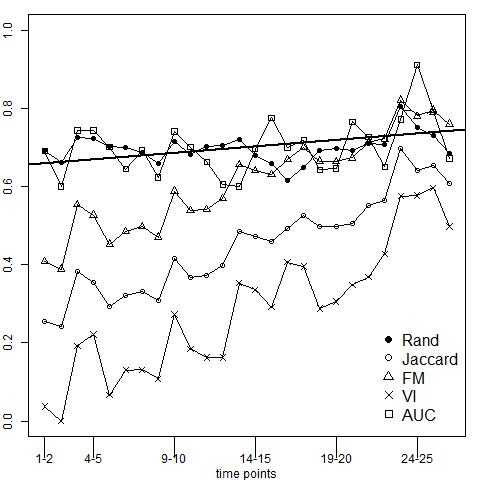
\includegraphics[width=0.45\textwidth]{images/chapter4/game27_cmeansClusters_Cons.png}
        }
        \subfigure[Hirarchical Clustering]{
            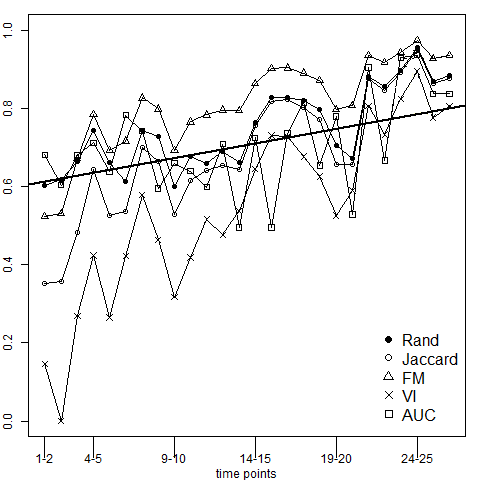
\includegraphics[width=0.45\textwidth]{images/chapter4/game27_hierClusters_Cons.png}
        }\\
        
    \end{minipage}}
    \caption{Results of various clustering methods using the previous time point as reference of behaviour to calculate the magnitude of changes which happen to the groups of items in consequent time points in the 27 rounds PGG data set.}
    \label{fig:game27_ChangeMeasuers_Cons}
\end{figure}
    
\subsection{Using MONIC}
    
We used MONIC\footnote{Available at http://infolab.cs.unipi.gr/people/ntoutsi/monic.html} to gain more insight into the public goods games data and to compare our results with the existing methods of measuring cluster changes in different time points. The data for each time period were clustered separately using k--means with four clusters. The clustering was carried out on the main temporal attributes of the data, namely belief and contribution. Then the data and cluster labels of items in each consequent pair of time points were fed to the MONIC algorithm to calculate changes to clusters from one time point to another. The method calculated the number of survived, appeared and disappeared clusters, as shown in figures \ref{fig:monic10} and \ref{fig:monic27}, for the ten rounds of the game.
    
    
In the 10 rounds data set, the number of survived clusters reduced from four clusters between the first and second time points until it reached zero, while new clusters appeared in the middle of the fifth and sixth game rounds. Then the number rose again until the end of the game. This might be due to the fact that players are changing their strategies and exploring new options until they ultimately settle on a certain strategic pattern. This change is consistent with our findings, as the measures slightly increase between the fifth and seventh time points, which might be an indication of players changing their strategy back to their original one. As Keser and Winden \cite{Keser2000} suggest, this change might be due to the players responding to the average contribution of other players in the previous round.
    
\begin{figure}[!h]
    \centering
    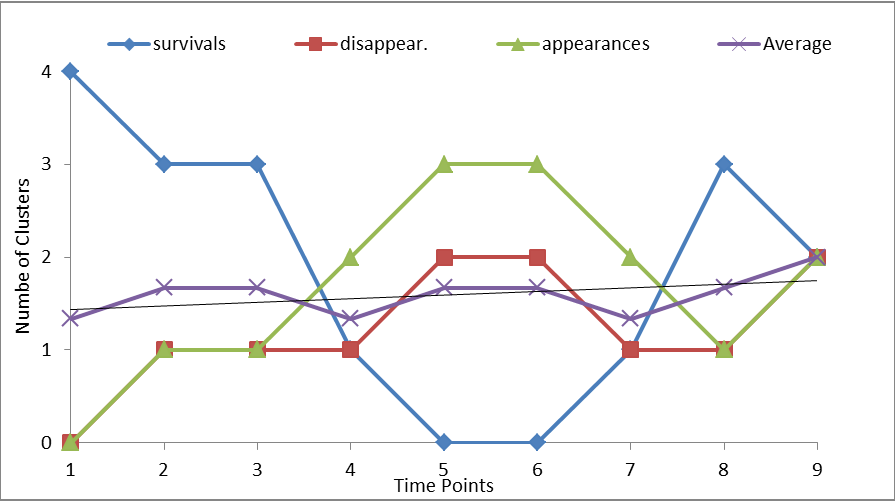
\includegraphics[width=0.75\textwidth]{images/chapter4/monic10.png}
    \caption{Number of survival, appearance and disappearance of clusters between every tow consequent time points for ten rounds public goods game as measured by MONIC.}
    \label{fig:monic10}
\end{figure}

The results for the 27 rounds data set is not straightforward as the numbers of cluster survivals, appearances and disappearances change more frequently. However, the cyclic pattern of increasing and decreasing number of survived clusters might be an effect of changing players' strategies or due to the underlying algorithm, as it provides an ageing factor to the items.

\begin{figure*}[th]
    \centering
    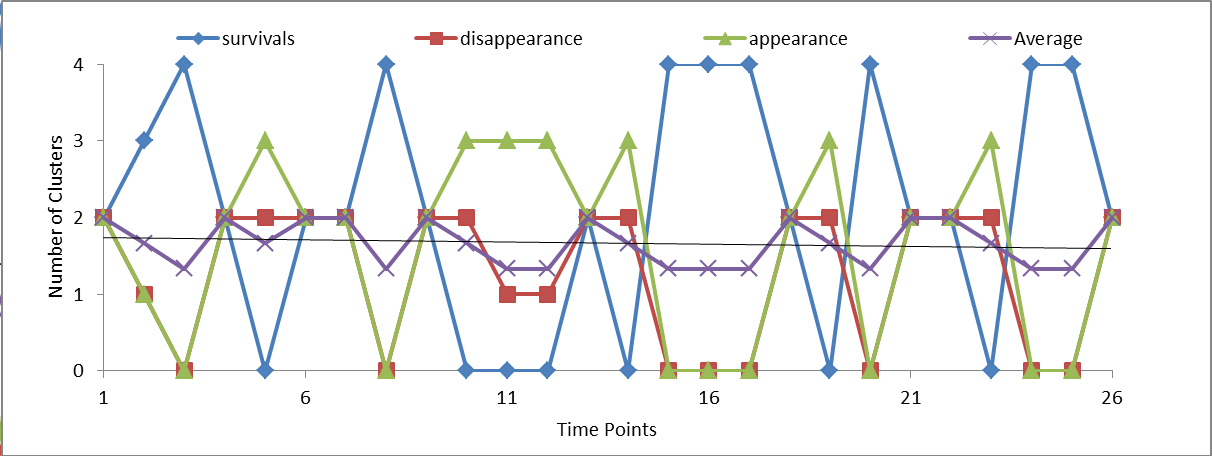
\includegraphics[width=1.0\textwidth]{images/chapter4/monic27.png}
    \caption{Number of survival, appearance and disappearance of clusters between every tow consequent time points for 27 rounds public goods game as  measured by MONIC.}
    \label{fig:monic27}
\end{figure*}

As the MONIC algorithm was originally introduced to detect cluster changes in data streams, it uses an ageing factor which reduces the effect of older items in the cluster and removes items older than two time points \cite{Spiliopoulou2006}. This ageing factor is essential for the algorithm to keep up-to-date with the flowing data stream and provide the right results for the current status of the clusters. However, this might not be useful for public goods games data, as there is a fixed number of players. This might result in the removal of players who stay in the same cluster for long time points. The effect of the ageing might not be obvious in the 10 rounds game due to the limited number of time points, but it might still undermine players' strategies.
                                 
While the proposed method assumes a fixed number of clusters to calculate the change in items membership, the MONIC algorithm is an effective method for gaining insights into the available clusters and their stability by measuring the number of survived clusters between two time points. However, it does not measure a number of items drifting from one cluster into another, which can be detected by the proposed method, as it introduces a specific ratio between each consequent time point, indicating the amount of change was happening to the items in the clusters by calculating their membership change among clusters.
                                 
MONIC can be compared with the proposed method especially the case of previous time point as a reference of behaviour as both of these methods compare the current clusters with the previous time point. The regression result for the average of cluster moves (appear, disappear and survive) is near to zero, which is compatible with the proposed method results using the previous time point as a reference of behaviour except for 27 rounds clustered by PAM and hierarchical clustering. By comparing results from the proposed method and MONIC, we can conclude that the players slightly and gradually change their cluster membership. However, the magnitude of change is stable from one time point to another. The proposed method provides an exact number for the change while the MONIC presents overall clusters movement and change.
                                 
\section{Summary}

The primary purpose of this chapter is to answer two of the main questions of the study. The first question is: Can we use the proposed method in chapter three to measure changes over time? The second question is: Do players of PGG behave as predicted by economists? As presented in chapter three, the proposed method consists of two main steps. The first step is to cluster items at each time point,  and the second step is to measure changes happening in the clusters of each time point using a reference of behaviour. Many types of reference of behaviour for items in the data set can exist; in this chapter, we tested two, namely the first time point and previous time point.

To answer the first question we checked the validity of hypothesis  \ref{hypo:diffCluster} and \ref{hypo:diffCVI}. Laid out in the first chapter, they are:
\begin{itemize}
    \item To prove that the above proposition is valid the results of different external clustering indices and AUC should be consistent.
    \item Using different clustering algorithms will not produce a significant difference in the final result of quantifying the changes over time as long as same clustering algorithm is used at both time points.
\end{itemize}
These two hypotheses examine the main aspects of the proposed method for measuring items' changes over time in temporal data. If these two hold true, then they can be presented as evidence which proves that the proposed method is working adequately and consistently.


To check the validity of these two hypotheses, we used the synthetic data which was introduced in chapter three. Prior to the experiment of testing the proposed method, the rationale for selecting certain clustering methods and external cluster validity indices is presented. It is crucial to make sure that the appropriate range of clustering methods are used so that items at each time point are clustered appropriately. We chose clustering methods which mainly separate items according to their distance from each other; the clusterings used are k--means, c--means, PAM and hierarchical clustering for this purpose. For external cluster validity indices,  we have mainly used the matching based methods of Jaccard Coefficient, Rand Statistic and Fowlkes-Mallows Measure. We have also used the Variation of Information VI method, which is an example of a statistical-based model, and AUC of ROC with players to measure the efficiency of classification.

Tests of the synthetic data using the proposed method with suggested clustering and external cluster validity indices multiple sample sets of results are produced. By using p-value for Wilcoxon-test, we demonstrated that each pair of results is similar to each other except for some hierarchical clustering cases. This similarity proves that the results of proposed method are consistent regardless of the clustering method used. This, therefore, verifies the validity of hypothesis  \ref{hypo:diffCluster}. While the similarity between different external cluster validity indices did not hold true, each external cluster validity indices result, however, proved to be similar across different clustering algorithms meaning the results of the external cluster validity indices are consistent but with different sensitivities to the change of items. After conducting these tests, it can be concluded that the proposed method can be successfully used to measure and quantify changes of items in temporal data.

To answer the second question, we used the proposed method on both PGG data sets introduced in chapter three. The same choice of clustering methods and external cluster validity indices are used in the process of quantifying players' strategy change. Four clusters are used of players in each time point because economists have categorised players into four groups in their studies. The four-cluster model was a viable choice as we tested the data using the Elbow method to determine the number of clusters in the data sets. The results showed that the players' strategy change when approaching the end of the game. However, the change itself between any two time point is constant on average. This result corresponds with economists' conclusions.


To gain another perspective on the players' strategy change, we used the MONIC method which was created to detect cluster change in data streams. The results showed that the clusters periodically appear and disappear through data points in the temporal data of PGG. This is an indication that the players' strategy changes as new clusters are emerging and others vanishing. Moreover, the unstable number of survived clusters is an indication that the players are not changing their strategy homogeneously and their reaction varies from each other. While the MONIC method provides a new perspective on the data set, however, it is not possible to directly compare it with the results of our proposed method because they consider different aspects of the data. The proposed method quantifies the amount of individual items exchange between clusters while MONIC shows the changes which are happening to the clusters in general.

In this chapter, we made a comparison between two different references of behaviour for items in temporal data, namely the first time point and the previous time point of the temporal data set. However, another reference of rehavior is proposed in chapter three which is the  general behaviour across all time points. This type of reference of rehavior is possible if the class of each item is known in the temporal data. In chapter five, we propose a new algorithm to classify items in a temporal data by optimising rules for classes provided by experts or human agents. In chapter six, we will use the produced classes of items as the reference of rehavior to measure changes in items.
